\section{sandman2}\label{sandman2}

Sandman2 je nástroj, který automaticky poskytuje REST API nad SQL databází \autocite{sandman}. Stačí mu předat údaje k~databázi a je možné jej hned začít používat. Je možné jej spustit jako samostatnou službu nebo jej integrovat do vlastní aplikace. Ve výchozí konfiguraci zpřístupní celou databázi, toto chování lze ale změnit a zpřístupnit jen část, případně u~některých tabulek povolit jen některé operace. Příklad úpravy můžete vidět \protect\hyperlink{code:sandman}{v~ukázce}.

\begin{listing}[htbp]
\caption{{\label{code:sandman}sandman: Příklad úpravy chování \autocite{sandman1gh}}}
\begin{minted}[bgcolor=codebg]{python}
class Style(Model):
    """Model mapped to the "Genre" table

    Has a custom endpoint ("styles" rather than the default, "genres").
    Only supports HTTP methods specified.
    Has a custom validator for the GET method.

    """

    __tablename__ = 'Genre'
    __endpoint__ = 'styles'
    __methods__ = ('GET', 'DELETE')
    __top_level_json_name__ = 'Genres'

    @staticmethod
    def validate_GET(resource=None):
        """Return False if the request should not be processed.

        :param resource: resource related to current request
        :type resource: :class:`sandman.model.Model` or None

        """

        if isinstance(resource, list):
            return True
        elif resource and resource.GenreId == 1:
            return False
        return True
\end{minted}
\end{listing}

Sandman2 používá Flask a SQLAlchemy, takže podporuje širokou škálu SQL databází včetně MySQL, PostgreSQL, Oracle, Microsoft SQL Serveru a SQLite \autocite{sandmangh}. Závisí přímo na čtyřech a nepřímo na dvanácti modulech, instalace má celkem 82~207 řádků kódu a tím -- v~negativním slova smyslu -- předčí všechny ostatní frameworky.

Kromě samotného REST API vytvoří sandman2 i webové rozhraní, kde je možné s~daty manipulovat. Můžete jej vidět \protect\hyperlink{pic:sandman}{na obrázku}.

\begin{figure}
\centering
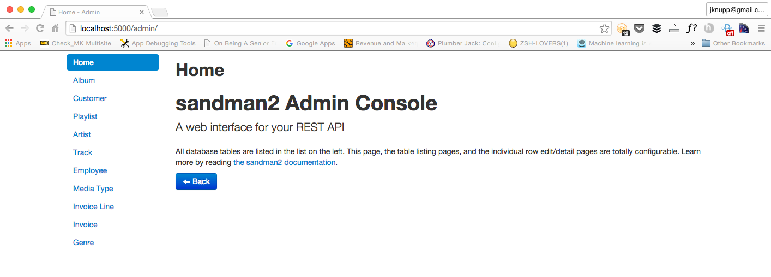
\includegraphics{images/sandman}
\caption{sandman2: Webové rozhraní \autocite{sandmanpic}\label{pic:sandman}}
\end{figure}

Sandman2 je pokračovatelem projektu sandman \autocite{sandman1}, který je momentálně opuštěný a obsahuje informaci o~tom, že by uživatelé měli používat druhou verzi \autocite{sandman1gh}. Sandman2 ale nemá tak obsáhlou dokumentaci jako sandman. Původní sandman vznikl v~roce 2013 a vyšlo celkem 45 verzí, sandman2 je zde od roku 2014, verzí vyšlo sedm, poslední v~lednu 2016. Za sandmenem stojí jednotlivec Jeff Knupp, do projektu přispělo několik jednotek dalších přispěvatelů. Na GitHubu má sandman2 pouze 128 hvězd, ale sandman jich má přes dva tisíce.

\subsection{HATEOAS}\label{hateoas}

Sandman automaticky prezentuje SQL sloupce typu cizí klíč jako odkazy \autocite{sandman1gh}. Předpokládám, že sandman2 to dělá stejně, ale tuto informaci jsem nikde nenašel potvrzenou. Dávám zde tedy dva body na základě vlastnosti z~první verze sandmanu.

\subsection{Přístupová práva}\label{pux159uxedstupovuxe1-pruxe1va}

Dokumentace k~původnímu sandmanu uvádí, že je možné použít HTTP autentizaci jménem a heslem a na základě ní zpřístupnit celé API pouze přihlášeným uživatelům \autocite{sandmanauth}. Jiné zabudované možnosti podporovány zatím nejsou. Je ale možné napsat speciální funkci, která předzpracovává všechny požadavky a v~této implementovat jiný způsob autentizace a autorizace.

Sandman2 informace o~přístupových právech v~dokumentaci neobsahuje, tato funkcionalita zde ještě není; dostává tedy nula bodů.

Sandman2 je nástroj, který mapuje REST rozhraní k~SQL databázi a dělá to dobře. Nepříjemný je přerod projektu sandman do projektu sandman2, na který doplácí hlavně dokumentace, což se doufám časem zlepší.
